\documentclass[../PS6_RapportFinal.tex]{subfiles}

\begin{document}
\graphicspath{{img/}{tex/img/}}
\subsection{Essais}

Une fois l'échangeur réalisé, nous avons procédé à divers tests. Tout d'abord, nous avons vérifié que celui-ci était effectivement étanche. Suite à cet essai, nous nous sommes aperçu que les raccords d'entrée/sortie d'eau, ainsi que la jonction pieux/raccords présentaient des fuites. Pour les raccords de connexion au réseau hydraulique, nous avons réalisé une soudure à froid par dessus celle déjà effectuée, tandis que pour les pieux nous avons réalisé des joints en silicone en plus de ceux en colle déjà présents.

\begin{figure}[!h]
\begin{center}
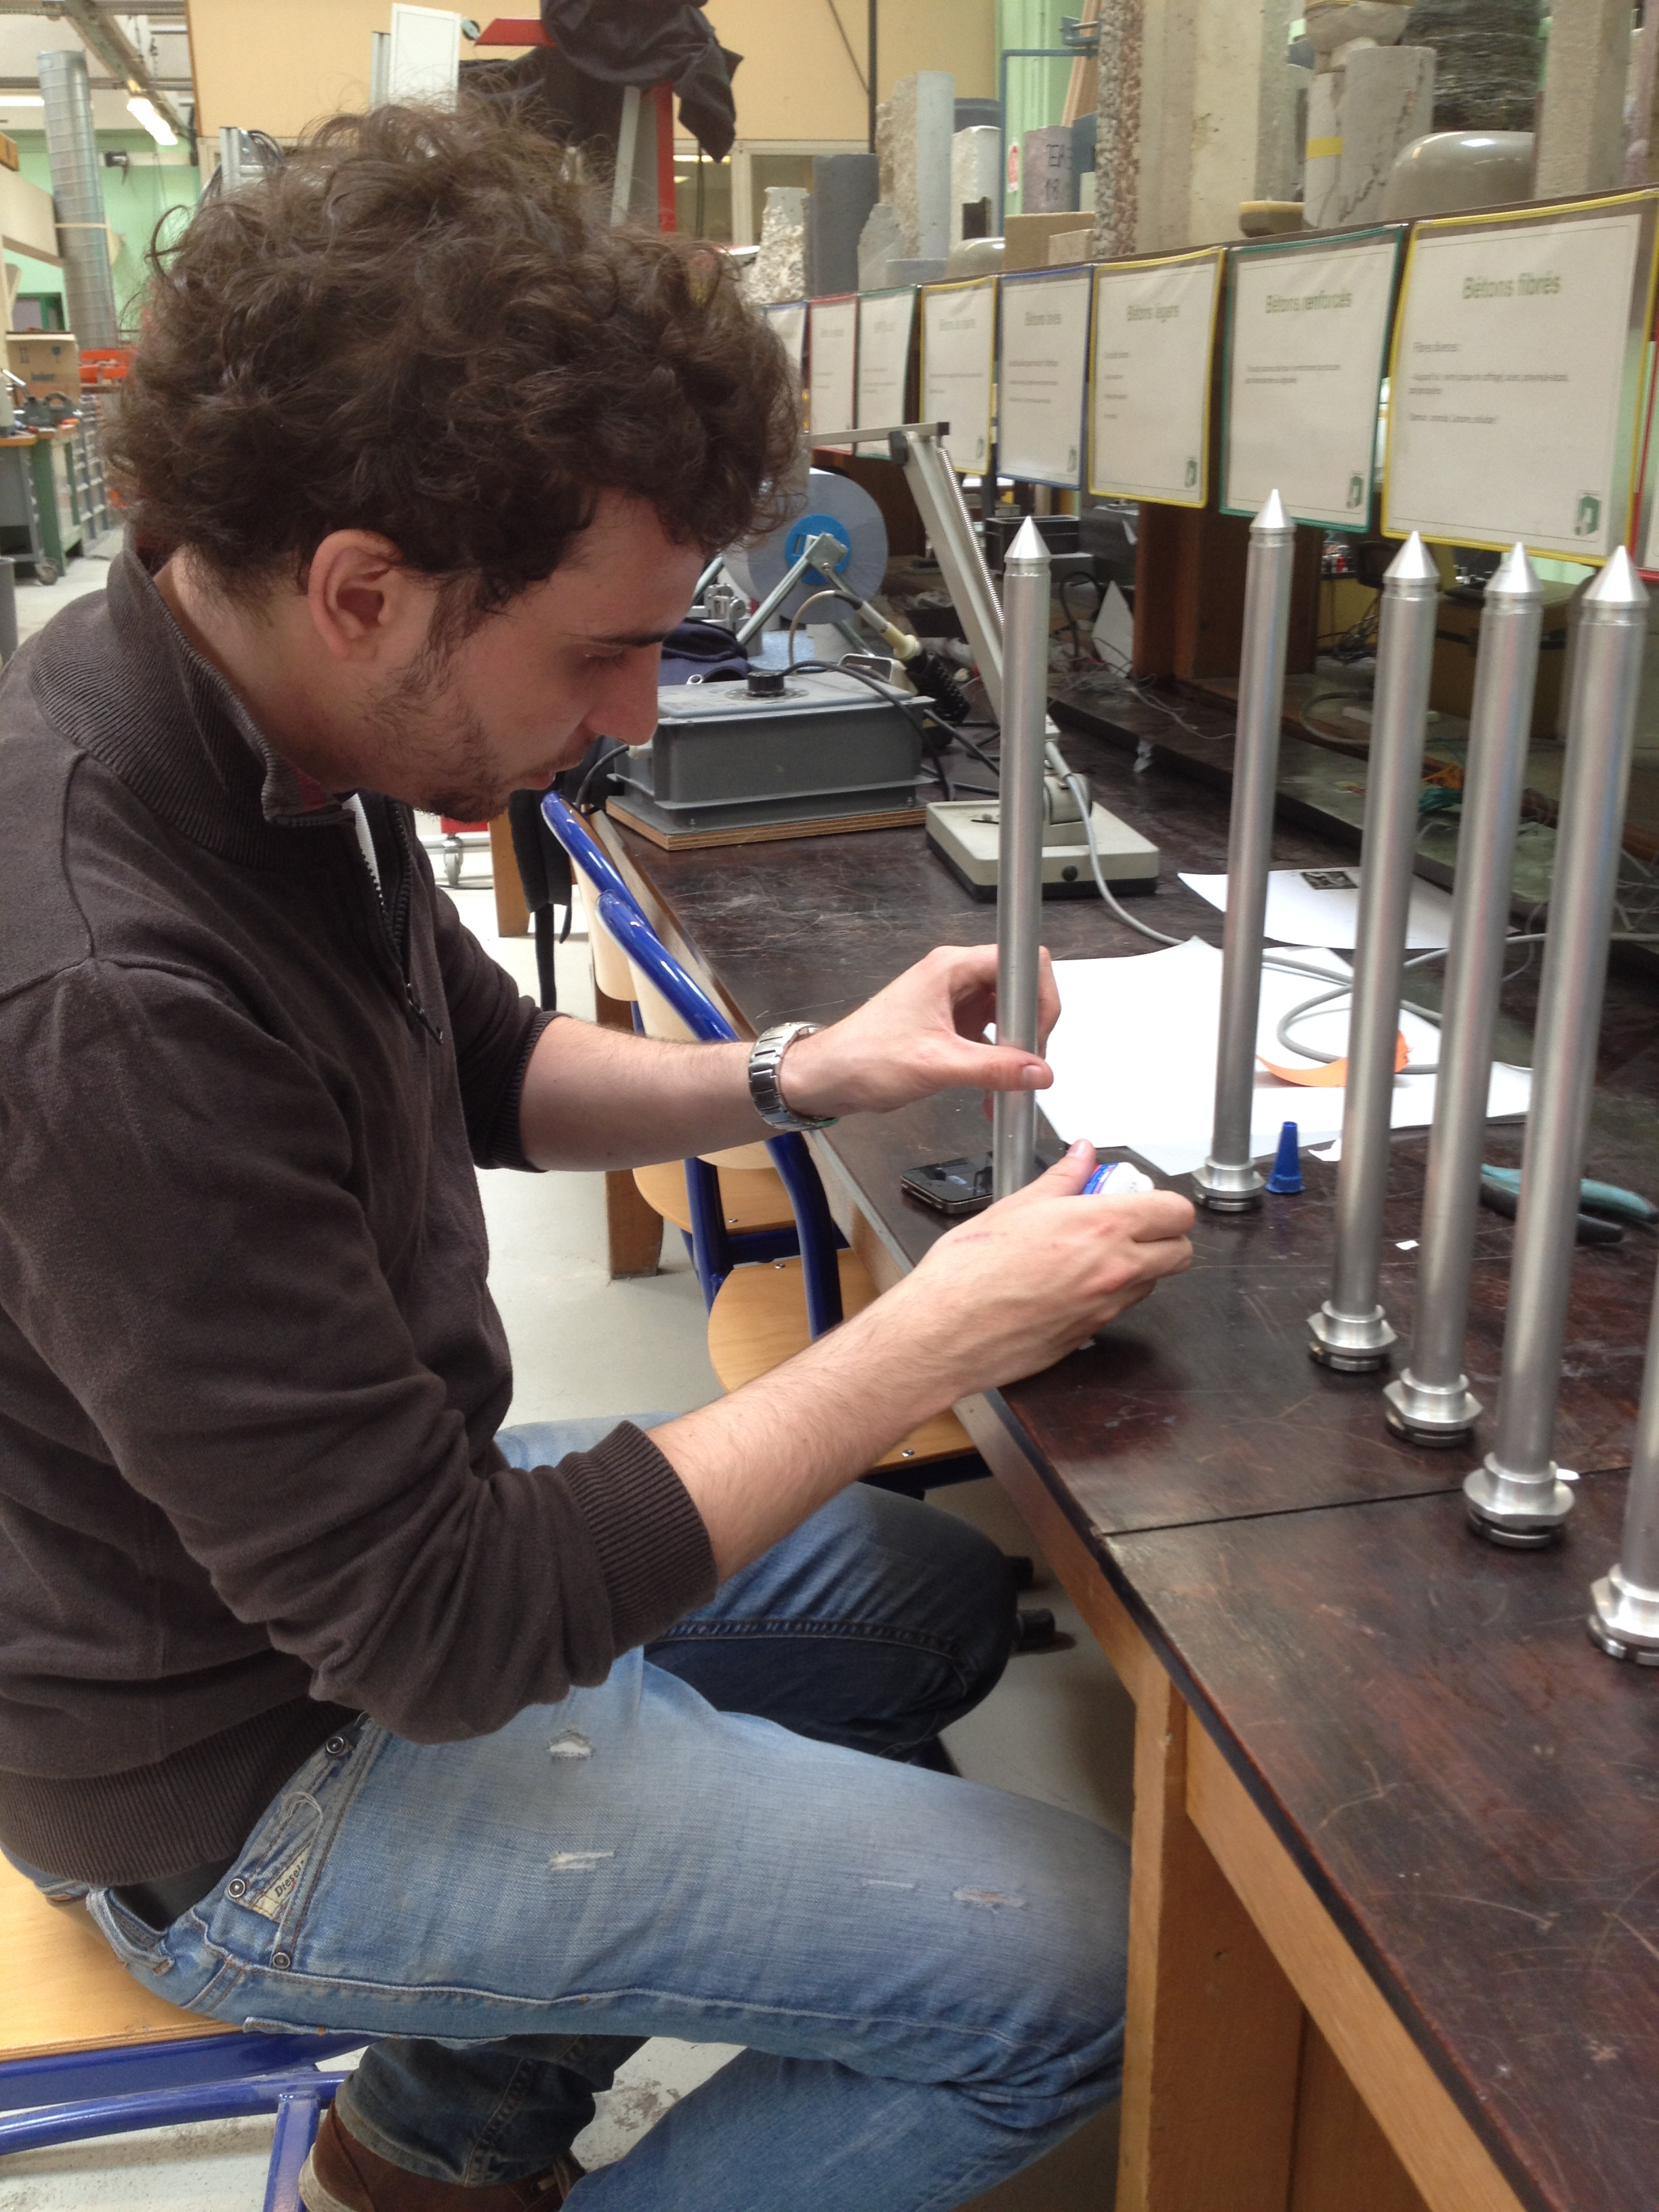
\includegraphics[height=7cm]{3_1_photo1.jpg}
\caption{Collage des raccords}
\end{center}
\end{figure}

Une fois l'échangeur totalement étanche, nous avons effectué un essai de plantage dans les cuves : nous n'avons rencontré aucun problème particulier et le dispositif se plante assez facilement. 

\begin{figure}[!h]
\begin{center}
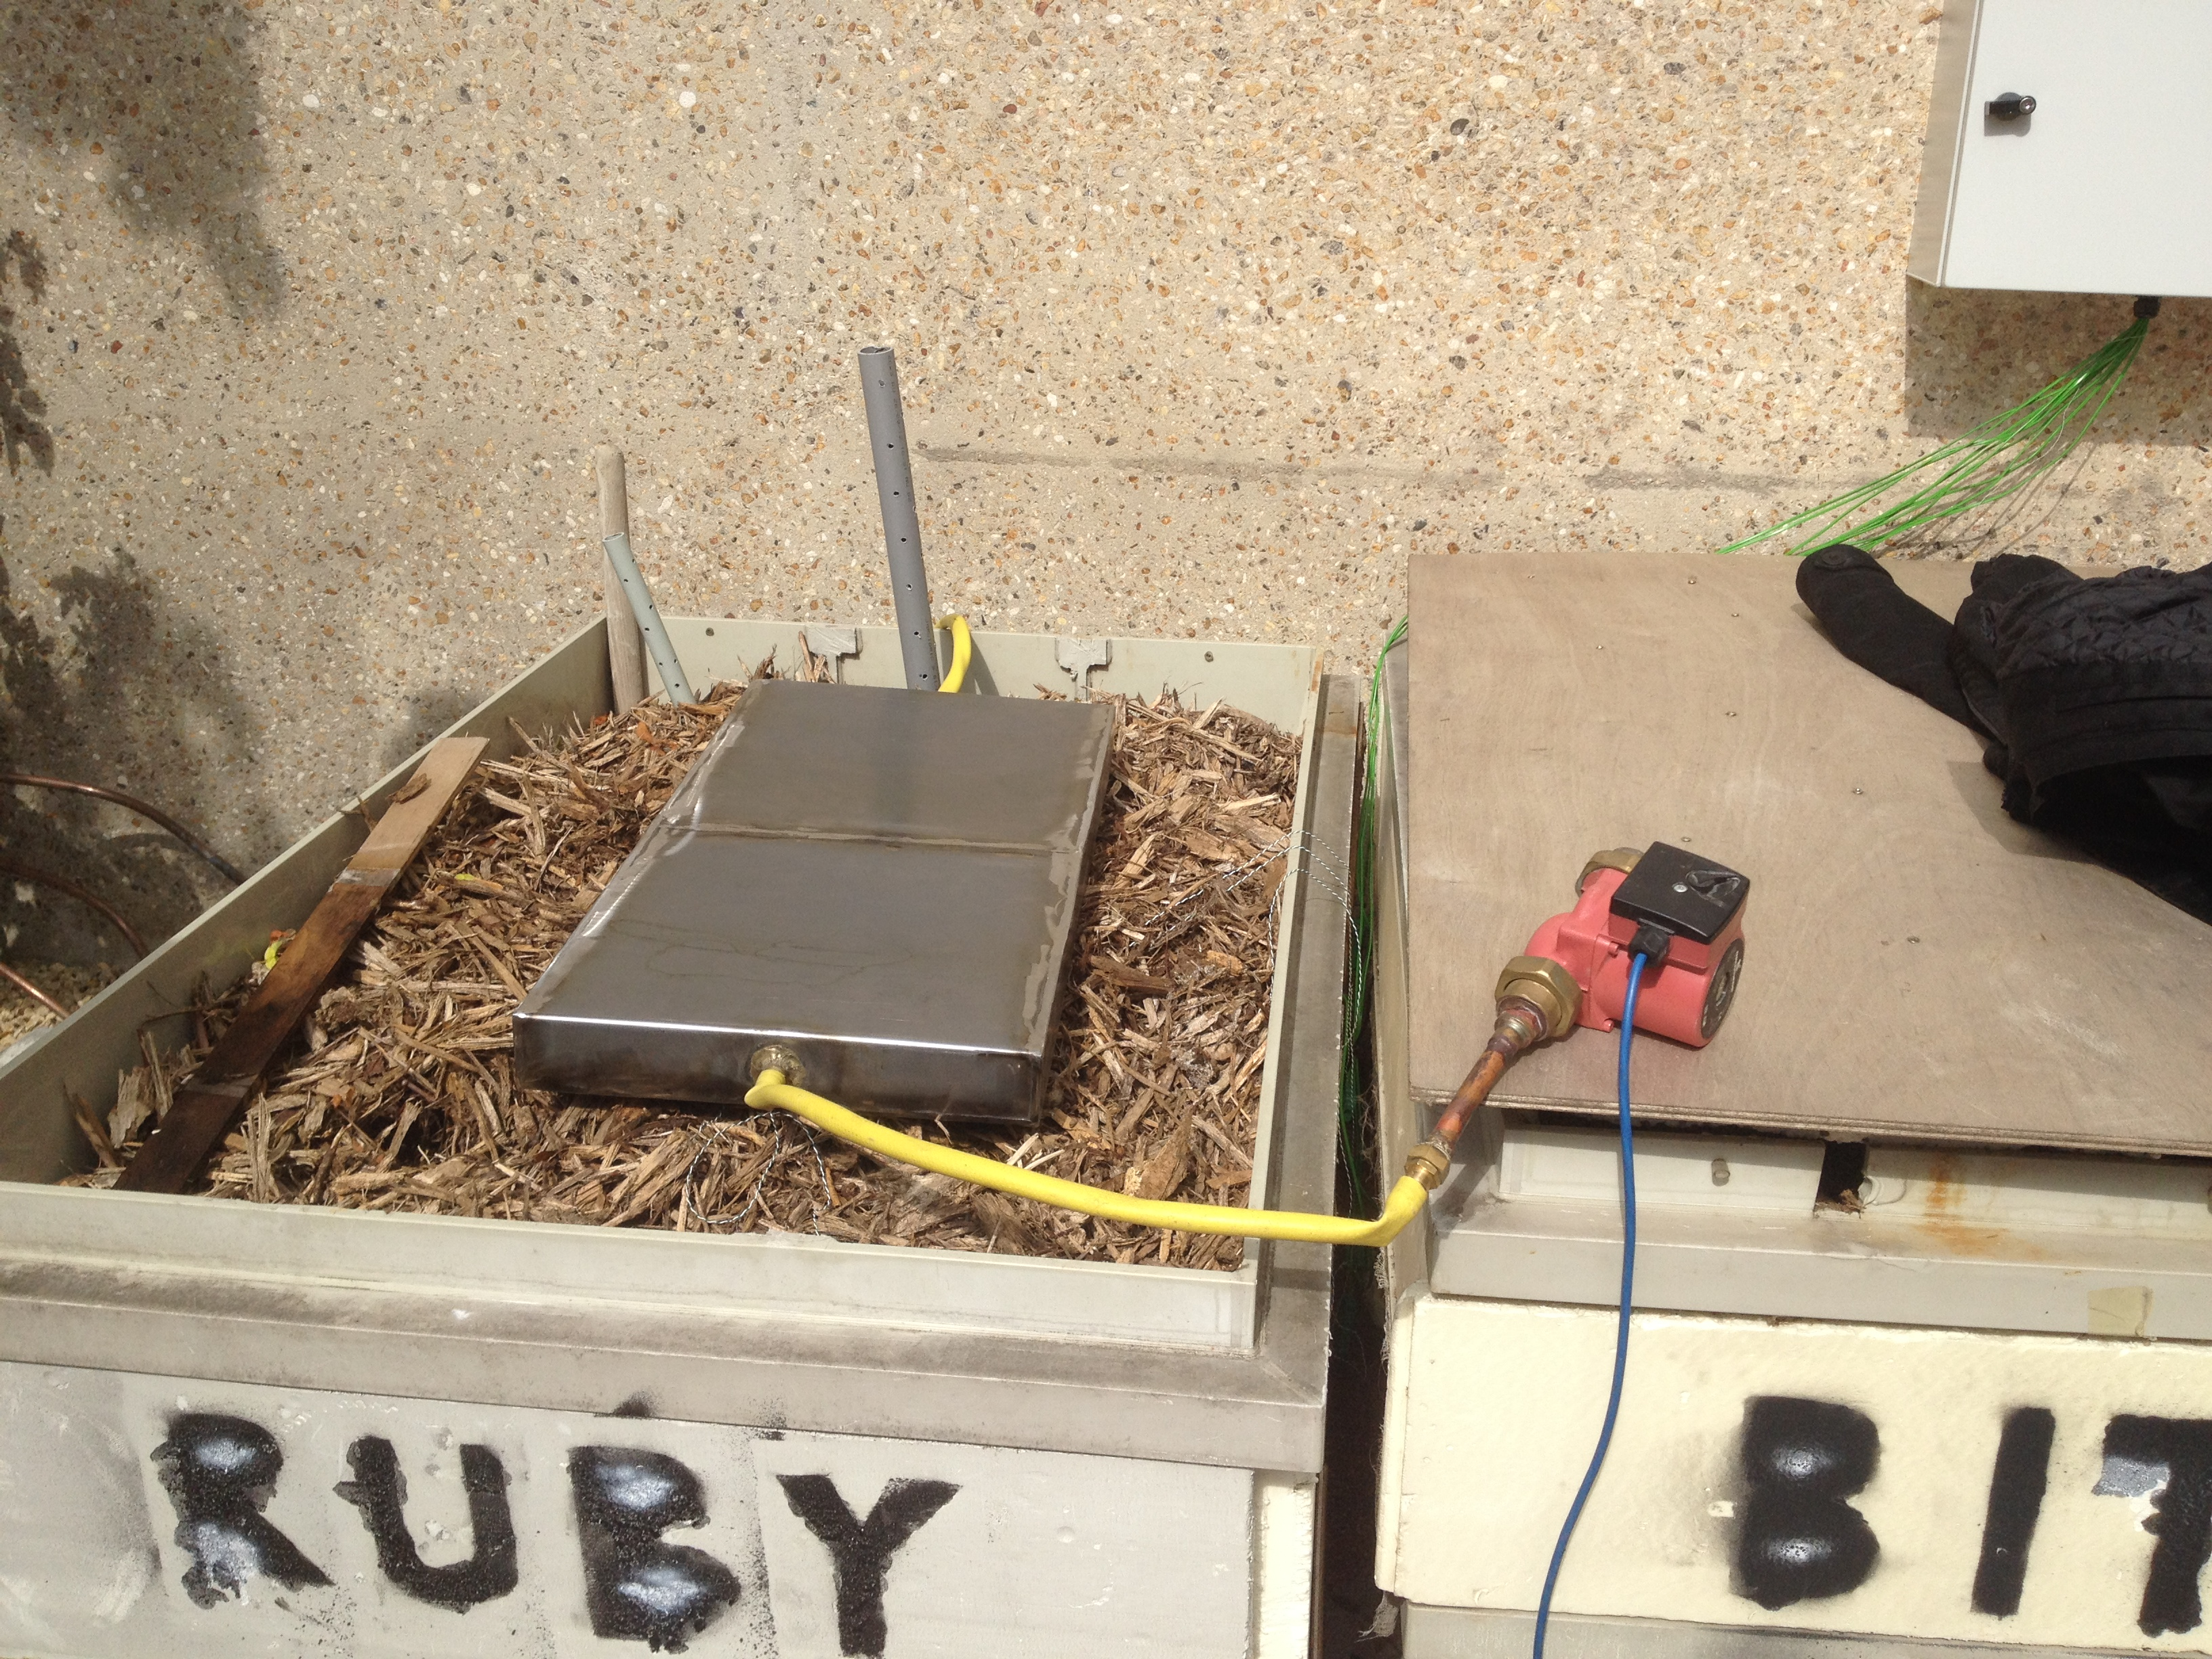
\includegraphics[width=10cm]{3_3_Plantage.jpg}
\caption{Premier essai de plantage}
\end{center}
\end{figure}

Suite à ceci, nous avons effectué des relevés de température en faisant fonctionner \og à vide\fg{} l'échangeur. Celui-ci baignait dans une cuve thermostatée remplie d'eau. L'accouplement au réseau hydraulique était relié à un robinet dont nous avons mesuré le débit (5\si{\liter\per\minute}), et l'autre débouchait, via un tuyau, dans un seau. Nous avions par ailleurs placé des thermocouples, reliés à un boitier d'acquisition, au niveau de la sortie d'eau, à l'intérieur du bain, et avions mesuré la température d'entrée dans l'échangeur.

\begin{figure}[!h]
\begin{center}
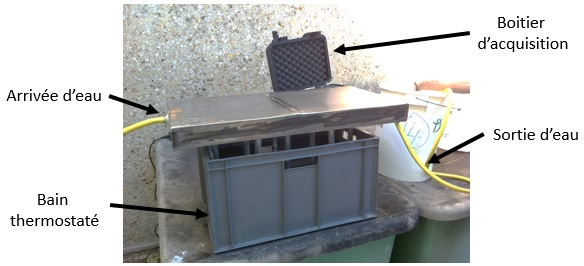
\includegraphics[width=10cm]{3_3_Dispositif_essais.jpg}
\caption{Banc de mesures}
\end{center}
\end{figure}
\vspace{1\baselineskip}

Suite à cette expérimentation, nous avons obtenu les courbes suivantes :

% Mesures

On définit l'efficacité thermique de l'échangeur comme suit :

\[\varepsilon = \frac{\Phi _{haut}}{\Phi _{bas}}\]

avec 
\begin{itemize}
\item \(\Phi_{haut} = \rho  Q_V c_P(T_S - T_E)\)
\item \(\Phi_{bas} = U_{pieu} (T_{compost} - T_E)\)
\item \(U_{pieu} = h_{ext}+h_{int}+\frac{\lambda 2\pi L}{\ln (\frac{r_2}{r_1})}\)
\end{itemize}

Le coefficient d'échange surfacique entre le compost et le tube du caloduc n'est pas le même que celui entre l'eau utilisée pour l'expérience et le caloduc.
C'est ce que l'on constate sur la figure \ref{caracech} qui représente la température dans l'échangeur en fonction du flux, pour différents coefficient d'échange surfacique.

\begin{figure}[!h]
\begin{center}
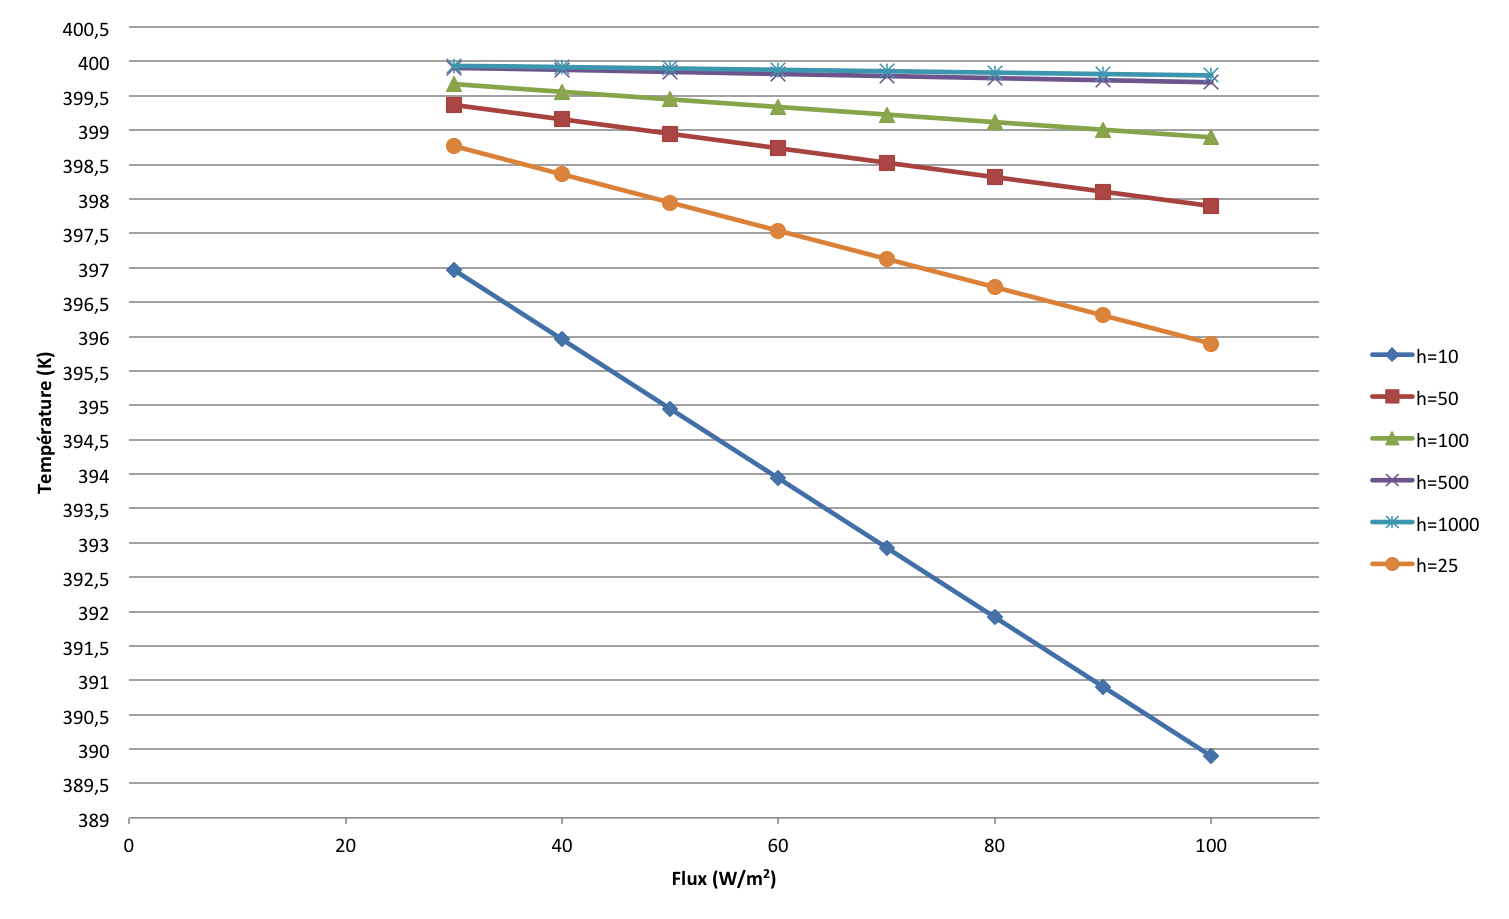
\includegraphics[width=8cm]{3_3_caracech.png}
\caption{Caractérisation de l'échangeur}
\label{caracech}
\end{center}
\end{figure}

On introduit alors un facteur correctif \[\alpha =\frac{\varepsilon _{réel}}{\varepsilon _{exp}}=\frac{\Phi _{bas-exp}}{\Phi _{bas-réel}}=\frac{h_{ext}+ h_{int}+\frac{\lambda 2\pi L}{\ln (\frac{r_2}{r_1})}}{2 h_{int}+\frac{\lambda 2\pi L}{\ln (\frac{r_2}{r_1})}}\]

\begin{multicols}{2}
On relève
\begin{itemize}
\item \(T_E = \num{298.5} \si{\kelvin} \)
\item \(T_S = \num{302.5} \si{\kelvin}\)
\item \(T_{eau} = \num{316.25} \si{\kelvin}\)
\end{itemize}
\columnbreak
Et on a 
\begin{itemize}
\item \(r_2 = 11\si{\milli\metre} \)
\item \(r_1 = \num{9.5}\si{\milli\metre} \)
\item \(\rho = 1000 \si{\kilo\gram\per\cubic\metre} \)
\item \(Q_V = \num{2.31e-4}\si{\cubic\metre\per\second} \)
\item \(\lambda = 237 \si{\watt\per\cubic\metre\per\kelvin}\)
\item \(h_{ext} = 10 \si{\watt\per\cubic\metre\per\kelvin} \)
\item \(h_{int} = 1000 \si{\watt\per\cubic\metre\per\kelvin}\)
\item \(L = \num{0.78} \si{\metre}\)
\end{itemize}
\end{multicols}
Et donc 
\(\alpha =\num{0.9002} \). Ainsi, \(\varepsilon =\num{0.216}\)

\end{document}